\documentclass{article}
\usepackage[a4paper, total={6in, 8in}]{geometry}
\usepackage{multicol,lipsum}
\usepackage[toc,page]{appendix}
\setcounter{secnumdepth}{3} 
\usepackage[english]{babel}
\usepackage[utf8x]{inputenc}
\usepackage[T1]{fontenc}
\usepackage{float}
\usepackage{pdfpages}
\usepackage{xcolor}

\usepackage{graphicx}	        % Enable for eps and pdf figures, if they occur
\usepackage{hyperref}           % Enable embedded hyperlinks.
\DeclareGraphicsExtensions{.pdf,.png,.jpg}
\usepackage{grffile} %per risolvere il problema di immagini con molti . prima dell'estensione
\hypersetup{
    colorlinks=true,
    linkcolor=blue,
    filecolor=magenta,      
    urlcolor=cyan,
}
 
\urlstyle{same}

\usepackage{listingsutf8}   		% Enable to use accent in Source code comment.
 \usepackage{listings}
 \usepackage{caption}
\usepackage{color}				% Eclipse style color
\definecolor{javared}{rgb}{0.6,0,0} % for strings
\definecolor{javagreen}{rgb}{0.25,0.5,0.35} % comments
\definecolor{javapurple}{rgb}{0.5,0,0.35} % keywords
\definecolor{javadocblue}{rgb}{0.25,0.35,0.75} % javadoc
 \definecolor{bkcolour}{rgb}{0.95,0.95,0.92}
\lstset{
%inputencoding=utf8/latin1,	% Enable to use accent in source code comment
%breaklines=true,				% Enable to avoid the source code exit the length of the page
%language=sh,
%backgroundcolor=\color{bkcolour},
%basicstyle=\ttfamily,
%keywordstyle=\color{javapurple}\bfseries,
%stringstyle=\color{javared},
%commentstyle=\color{javagreen},
%morecomment=[s][\color{javadocblue}]{#}{#},
%numbers=left,
%numberstyle=\tiny\color{black},
%stepnumber=2,
%numbersep=70pt,
%%%showstringspaces=false
}

%\usepackage[hmarginratio=1:1,top=32mm,columnsep=20pt]{geometry} % Document margins
%\usepackage[hang, small,labelfont=bf,up,textfont=it,up]{caption} % Custom captions under/above floats in tables or figures
%\usepackage{booktabs} % Horizontal rules in tables

\colorlet{punct}{red!60!black}
\definecolor{background}{HTML}{EEEEEE}
\definecolor{delim}{RGB}{20,105,176}
\colorlet{numb}{magenta!60!black}

\lstdefinelanguage{json}{
    basicstyle=\footnotesize\ttfamily,
    %numbers=left,
    numberstyle=\scriptsize,
    %stepnumber=1,
    numbersep=5pt,
    showstringspaces=false,
    %breaklines=true,
    %frame=lines,
    %backgroundcolor=\color{background},
    literate=
     *{0}{{{\color{numb}0}}}{1}
      {1}{{{\color{numb}1}}}{1}
      {2}{{{\color{numb}2}}}{1}
      {3}{{{\color{numb}3}}}{1}
      {4}{{{\color{numb}4}}}{1}
      {5}{{{\color{numb}5}}}{1}
      {6}{{{\color{numb}6}}}{1}
      {7}{{{\color{numb}7}}}{1}
      {8}{{{\color{numb}8}}}{1}
      {9}{{{\color{numb}9}}}{1}
      {:}{{{\color{punct}{:}}}}{1}
      {,}{{{\color{punct}{,}}}}{1}
      {\{}{{{\color{delim}{\{}}}}{1}
      {\}}{{{\color{delim}{\}}}}}{1}
      {[}{{{\color{delim}{[}}}}{1}
      {]}{{{\color{delim}{]}}}}{1},
}

\title{Web App curricula - Ingegneria Informatica Unifi} % Article title
\author{Francesco Ermini}
\date{\today} % Leave empty to omit a date

%\DeclareCaptionFormat{listing}{\rule{\dimexpr\textwidth+17pt\relax}{0.4pt}\par\vskip1pt#1#2#3}

\DeclareCaptionFont{white}{\color{white}} 
\DeclareCaptionFormat{listing}{\rule{\dimexpr\textwidth+17pt\relax}{0.4pt}\par\vskip1pt#1#2#3}
%\DeclareCaptionFormat{listing}{\hspace*{-0.4pt}\colorbox{gray}{\parbox{\dimexpr\textwidth-2\fboxsep+.8pt\relax}{#1#2#3}}} 
%\captionsetup[lstlisting]{format=listing,labelfont=white,textfont=white} 
\captionsetup[lstlisting]{format=listing, singlelinecheck=false,  labelsep=space}%font={sf}, margin=0pt, singlelinecheck=false, textfont=white, labelsep=space
\renewcommand\lstlistingname{Listing}
% Default fixed font does not support bold face
\DeclareFixedFont{\ttb}{T1}{txtt}{bx}{n}{8} % for bold
\DeclareFixedFont{\ttm}{T1}{txtt}{m}{n}{8}  % for normal

% Custom colors
\usepackage{color}
\definecolor{deepblue}{rgb}{0,0,0.5}
\definecolor{deepred}{rgb}{0.6,0,0}
\definecolor{deepgreen}{rgb}{0,0.53,0.70}
%\definecolor{deepgreen}{rgb}{0,0.5,0}

% Python style for highlighting
\newcommand\pythonstyle{\lstset{
aboveskip=10pt,belowskip=10pt,
tabsize = 2,
breakatwhitespace=false, %serve per farlo andare a capo quando hai molti tab
numberstyle=\tiny\color{purple},
showstringspaces=false,
breaklines=true,
language=Python,
basicstyle=\ttm,
otherkeywords={self},             % Add keywords here
keywordstyle=\ttb\color{javapurple},
emph={search, <, },          % Custom highlighting
emphstyle=\ttb\color{deepred},    % Custom highlighting style
stringstyle=\color{deepgreen},
frame=tb,                         % Any extra options here
numbers=left,
numberstyle=\tiny\color{black},
xleftmargin=17pt,
  framexleftmargin=17pt,
  framexrightmargin=17pt,
%stepnumber=2,
%numbersep=70pt,
}}


% Python environment
\lstnewenvironment{python}[1][]
{
\pythonstyle
\lstset{#1}
}
{}

% Python for external files
\newcommand\pythonexternal[2][]{{
\pythonstyle
\lstinputlisting[#1]{#2}}}

% Python for inline
\newcommand\pythoninline[1]{{\pythonstyle\lstinline!#1!}}



% Python style for highlighting
\newcommand\shellstyle{\lstset{
aboveskip=10pt,belowskip=10pt,
breaklines=true,
language=sh,
basicstyle=\footnotesize\ttfamily,
otherkeywords={},             % Add keywords here
keywordstyle=\ttb\color{black},
emph={GET,POST,DELETE,PUT},          % Custom highlighting
emphstyle=\ttb\color{black},    % Custom highlighting style
stringstyle=\ttfamily\color{red!50!brown},%frame=tb,                         % Any extra options here
showstringspaces=false ,          % 
frame=tb,                         % Any extra options here
xleftmargin=17pt,
  framexleftmargin=17pt,
  framexrightmargin=17pt,
}}

% Python environment
\lstnewenvironment{shell}[1][]
{
\shellstyle
\lstset{#1}
}
{}
% Python for inline
\newcommand\shellinline[1]{{\shellstyle\lstinline!#1!}}


\begin{document}
\maketitle

\section{Requirements}
Le funzioni che devono essere supportate lato amministratore sono:
\begin{itemize}
\item Caricamento dati relativi a ciascun insegnamento: codice (ob), nome (ob), CFU (ob),
SSD (ob), URL scheda insegnamento, periodo di erogazione, anno di
programmazione
\item Caricamento dei possibili percorsi con nome del percorso e descrizione
\item Specifica della struttura di ciascun percorso: gruppi di esami a scelta vincolata
\item Modifica e cancellazione di insegnamenti, percorsi e loro struttura
\end{itemize}
Le funzioni che devono essere supportate lato studente sono:
\begin{itemize}
\item Immissione dati studente (matricola, nome e cognome)
\item Visualizzazione dei possibili percorsi e loro descrizione
\item Scelta del percorso
\item Visualizzazione dell'elenco dei possibili esami per il percorso scelto con accesso al link della scheda insegnamento per ciascun esame
\item Scelta, per ciascun gruppo a scelta vincolata previsto dal percorso, degli insegnamenti all'interno del gruppo
\item Visualizzazione del piano di studi specificato
\item Creazione di PDF e file di uscita a descrivere il piano scelto
\end{itemize}
Tecnologie di realizzazione:
\begin{itemize} 
\item  PostgreSQL, 
\item  Python
\item  Flask
\end{itemize}




\begin{figure}[H]
  \begin{center}
   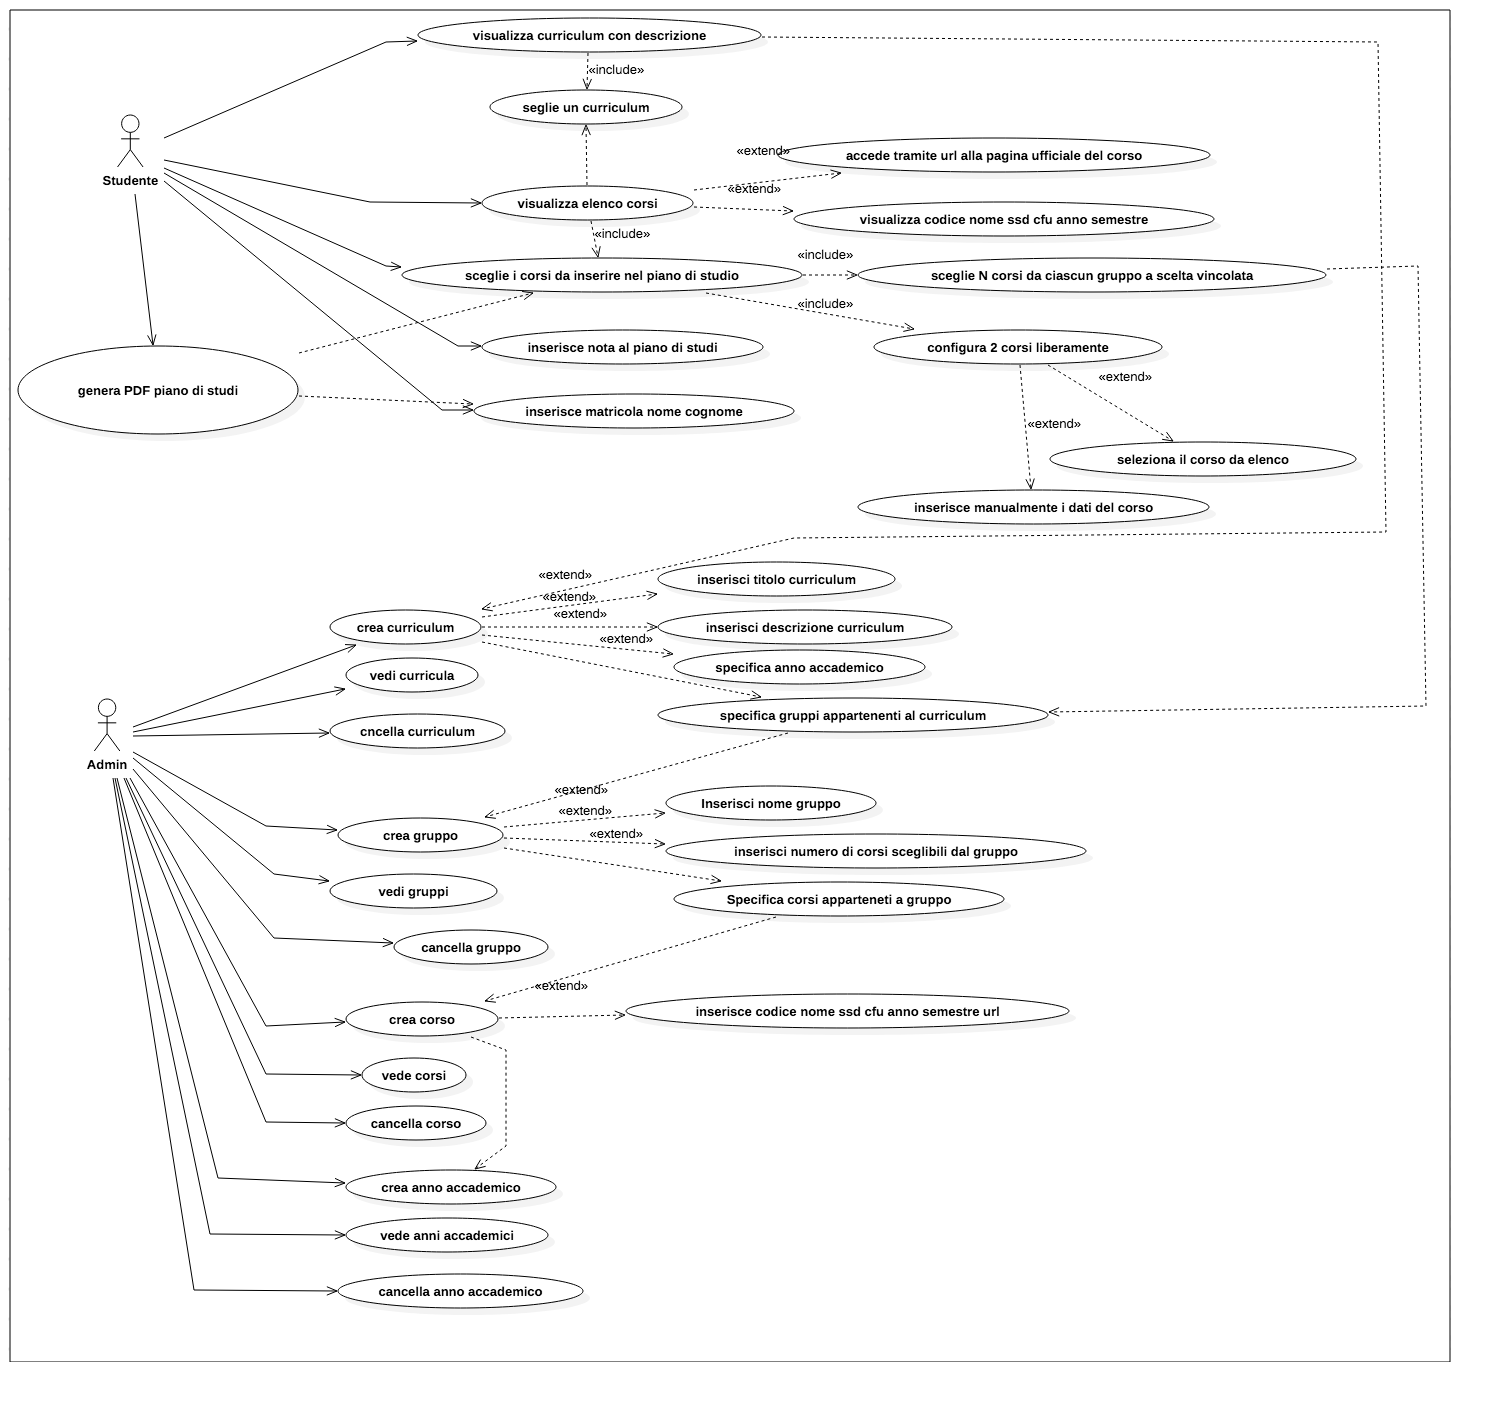
\includegraphics[width=\textwidth]{img/UseCaseDiagram.png}
     \caption{Use case diagram - simplified version}
  \label{fig:Usecasediagram}
  \end{center}
\end{figure}



\newpage
\section{Data model}
Dai requirements si sono  ricavate le seguenti entità:
\begin{itemize}
\item Student
\item Studyplan
\item Curriculum
\item Course
\item Group
\item Academicyear
\end{itemize}
\textbf{Student} consiste in una matricola (identificativo univoco di \emph{Student}), un nome e un cognome.
\\
\textbf{Studyplan} consiste in un curriculum ed un insieme non nullo di corsi scelti nel rispetto dei vincoli specificati dall'amministratore. L' \emph{id} è uguale alla matricola dello studente a cui appartiene.
\\
\textbf{Curriculum} consiste in un titolo, una descrizione, un anno accademico e un insieme non nullo di gruppi.
\\
\textbf{Group} consiste in un nome, un numero \emph{n} (numero di corsi da scegliere per quel gruppo),  un valore di \emph{cfu} e un insieme non nullo di \emph{Courses}. Rappresenta una  tabella di esami a scelta vincolata per un certo \emph{Curriculum}. 
\\
\textbf{Course} consiste in un codice corso (identificativo univoco del corso), un nome, un settore disciplinare, un numero di cfu, un anno accademico,  l'anno ed il semestre in cui è previsto lo svolgimento del corso ed un url alla pagina ufficiale del corso.
\\
\textbf{Academicyear} consiste in una stringa che rappresenta l'anno accademico (i.e 2018-2019), la data di inizio anno accademico e la data di fine anno accademico.


\begin{figure}[H]
  \begin{center}
   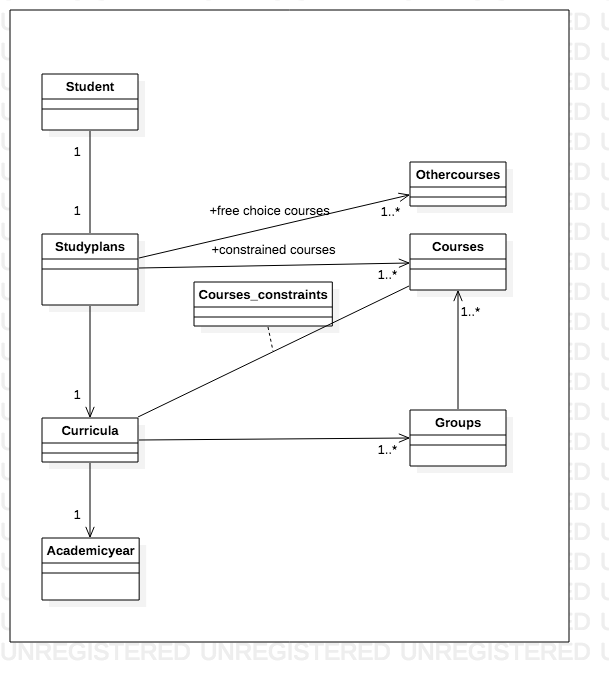
\includegraphics[width=.6\textwidth]{img/UMLconcettuale.png}
     \caption{UML concettuale}
  \label{fig:EntityRelationshipdiagram1}
  \end{center}
\end{figure}

Dai casi d'uso in \ref{fig:Usecasediagram} sono stati ricavate le relazioni mostrate in figura \ref{fig:EntityRelationshipdiagram1}
\begin{table}[!h]
  \begin{center}
    \caption{Entity relations}
    \label{tab:Entity Relationship}
    \begin{tabular}{l|l} % <-- Alignments: 1st column center, 2nd left
      \textbf{ER} & \textbf{cardinality}  \\ 
      \hline
		Student - Studyplans & one-to-one bidirectional \\
		Studyplans - Curricula & many-to-one bidirectional\footnote{La bidirezionalità da curriculum a piano di studi serve a permettere la cancellazione di un curriculum. Vedi note su cancellazione. } \\
		Studyplans - Courses  & many-to-many unidirectional \\
		Curricula - Groups & many-to-many unidirectional \\
		Groups - Courses & many-to-many unidirectional \\
    \end{tabular}
  \end{center}
\end{table}

In particolare si evidenziano le osservazioni:
\begin{itemize}
\item \textbf{Student - Studyplan}: Ad uno studente deve corrispondere uno e un solo piano di studi. Ad un piano di studi deve corrispondere uno e un solo studente. la relazione è stata modellata in modo bidirezionale, così che da uno studente si possa ricavare il suo piano di studi e viceversa. Se cancello uno studente  cancello il suo piano di studi e se cancello un piano di studi cancello lo studente a cui appartiene.
\item \textbf{Studyplan - Curricula }: Ad un piano di studio deve corrispondere uno e uno solo curriculum. Un curriculum è in uso su zero o molti piani di studio. Sebbene dai casi d'uso non sia emersa la necessità di sapere i piani di studio associati ad un curriculum, questa relazione è stata fatta bidirezionale per consentire l'eliminazione di un curriculum; Per cancellare un curriculum e non violare i vincoli di integrità  (foreign key su \emph{Studyplan}) è infatti necessario avere una relazione tra curriculum e piani di studio. Si sottolinea che così facendo l'eliminazione di un curriculum renda nullo il campo \emph{curriculum\_id} in tutti i piani di studio che lo avevano scelto. Questa opzione è stata considerata accettabile in fase di progettazione. D'altra parte l'amministratore deve avere totale controllo sulla eliminazione dei curricula. Inoltre se l'amministratore decide di eliminare un curriculum, i piani di studio che lo avevano scelto non saranno più validi.
\item \textbf{Studyplan - Courses}:  Ad un piano di studi devono corrispondere uno o più corsi. Un corso sarà incluso in zero o molti piani di studio.  La relazione è stata fatta unidirezionale perché non esiste un caso d'uso che richiede di sapere i piani di studio associati ad un corso. Quando l'amministratore elimina un corso, quel corso è automaticamente rimosso dai piani di studio che lo  avevano scelto.
\item \textbf{Curricula - Groups}: Un curriculum è fatto di uno o più gruppi. Un gruppo può essere incluso in zero o molti curricula. La relazione è stata fatta unidirezionale perché non esiste un caso d'uso che richieda di sapere i curricula associati ad un gruppo. L'eliminazione di un gruppo provoca la rimozione di quel gruppo dai curricula.
\item \textbf{Groups - Courses }: Un gruppo è fatto da uno o più corsi. Gruppi diversi possono avere alcuni corsi in comune (a patto che questi gruppi non appartengano ad uno stesso curriculum ). Anche in questo caso non esiste un caso d'uso che richieda di sapere, dato un corso, quali gruppi appartengono a quel corso.
\end{itemize}
La figura \ref{fig: Entity Relationship diagram 2} illustra il diagramma ER in prospettiva di implementazione.\\
Il database è stato realizzato in \texttt{Postgres} tramite \texttt{SQLAlchemy} in \texttt{Python Flask}.

\begin{figure}[H]
  \begin{center}
   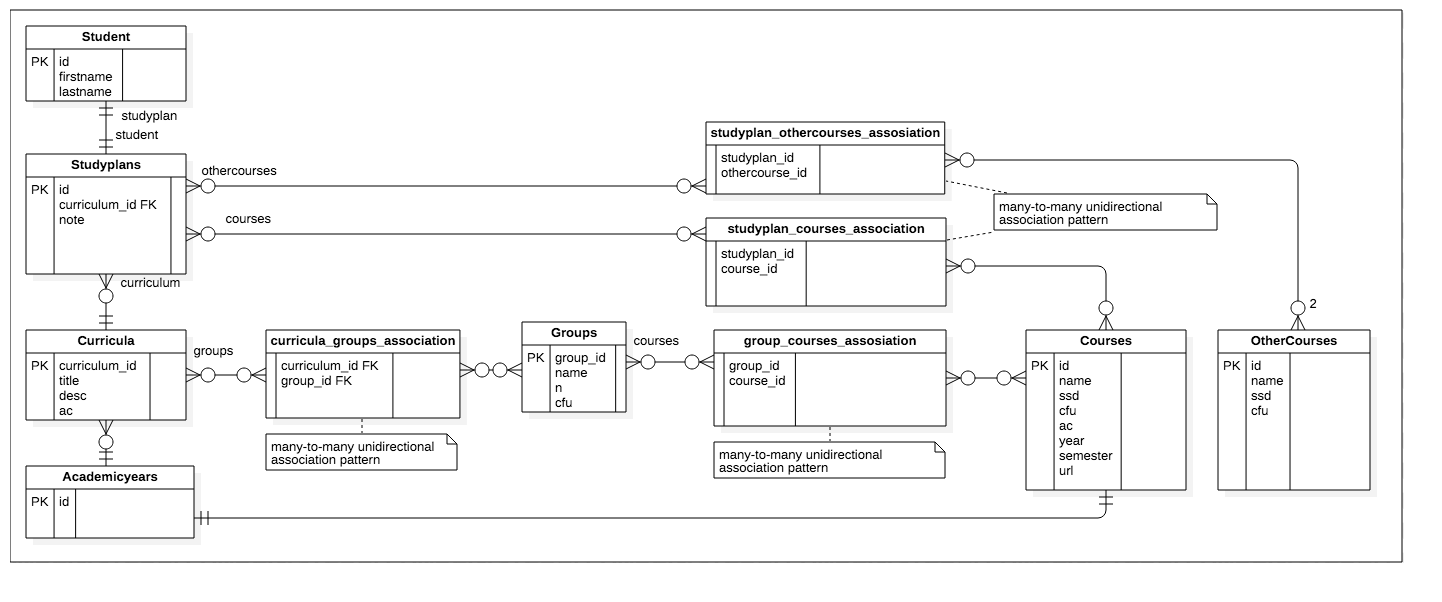
\includegraphics[width=\textwidth]{img/ERD.png}
     \caption{ER diagram 2}
  \label{fig: Entity Relationship diagram 2}
  \end{center}
\end{figure}



\section{Project Setup and structure}
Prima di procedere al setup assicurarsi di avere Python e pip installati. ( io ho python \textit{2.7.10} e pip \textit{18.0} ) 
\begin{shell}[caption=Setup Flask]
mkdir curriculaWebApp && cd curriculaWebApp
pip install virtualenv
virtualenv env
source env/bin/activate
git init
git clone https://github.com/FrancescoErmini/CurriculaWebApp2.git
export FLASK_APP=app.py
pip install Flask
pip install -r requirements.txt
\end{shell}
Poi dopo aver scaricato Postgres sul  proprio sistema operativo, accedere alla console \emph{psql}, quindi creare un database, creare un utente e associare utente al database.
\begin{shell}[caption=Create database]
CREATE USER pala WITH PASSWORD 'password';
CREATE DATABASE pianodistudio2;
GRANT ALL PRIVILEGES ON DATABASE pianodistudio2 TO pala;
\end{shell}
in alternativa, scaricare \textbf{pgAdmin 4} e fare tutto graficamente.\\
Prima di procedere oltre verificare che nel file \emph{app.py} i dati inseriti sopra siano corretti:
\begin{python}[firstnumber=16, caption=Flask db configuration]
POSTGRES = {
    'user': 'pala',
    'pw': 'password'
    'db': 'pianodistudio2',
    'host': 'localhost',
    'port': '5432',
}
app.config['DEBUG'] = True
app.config['SQLALCHEMY_DATABASE_URI'] = 'postgresql://%(user)s:\
%(pw)s@%(host)s:%(port)s/%(db)s' % POSTGRES
\end{python}
A questo punto si procede alla migrazione del database seguendo lo schema di migrazione \cite{ref1}. 
\begin{shell}[caption=Initialize database]
python manage.py db init
python manage.py db migrate
python manage.py db upgrade
python manage.py runserver
\end{shell}
Una volta avviato il server si può consumare le API sia da riga di comando che da interfaccia grafica.

\section{Validazione}



\subsection{validazione e vincoli sui dati}
La validazione del contenuto dei dati è utile per verificare i dati inviati tramite JSON post. In particolare \emph{ Academicyear, Course, Curriculum, Group} serviranno all'utente \textit{admin} per limitare l'inserimento di dati incorretti. Invece la validazione delle entità \emph{Student e  Studyplan} serviranno allo studente per controllare il rispetto dei vincoli.
\subsubsection{Academicyear}
Nel caso di \emph{ Academicyear} l'id è del tipo \texttt{2018-2019}.  La validazione consiste nel:
\begin{enumerate}
\item controllare che il valore sia non nullo
\item controllare che  il carattere '-' separi gli anni.
\item controllare che l'anno indicato si trovi in un range di valori ragionevoli, nel caso tra  2018 e 2022
\item controllare che l'anno successivo al primo sia quello successivo.
\end{enumerate}

\begin{python}
academicyear = data['id']
years = string.split(academicyear, '-')
if academicyear == "":
	return jsonify({"error":"Academic year can not be empty"}),500
if len(years) < 2:
	return jsonify({"error":"Wrong format. use minus char - to separate years"}),500
if int(years[0]) < 2018 or int(years[0]) > 2021:
	return jsonify({"error": "Year must be in range [2018,2021] "}),500
if (int(years[0]) + 1) != int(years[1]):
	return jsonify({"error": "Year not in format [<year>-<year+1>]" }),500
\end{python}

\subsubsection{Course}
Nel caso di \emph{Course} l'id è del tipo \texttt{B012345}. La validazione consiste nel
\begin{enumerate}
\item controllare che il valore sia non nullo
\item controllare che il codice abbia esattamente 7 caratteri
\end{enumerate}

\begin{python}
course_id = data['id']
if course_id == "":
	return jsonify({"error":"Course code can not be empty"}),500
if len(course_id) != 7:
	return jsonify({"error":"Course code is 7 char length"}),500
\end{python}


\subsubsection{Student}
Nel caso di \emph{Student} l'id è del tipo \texttt{1234567}. La validazione consiste nel
\begin{enumerate}
\item controllare che il valore sia non nullo
\item controllare che il codice abbia esattamente 7 caratteri
\end{enumerate}

\begin{python}
student_id = data['id']
if student_id == "":
	return jsonify({"error":"Student id can not be empty"}),500
if len(student_id) != 7:
	return jsonify({"error":"Student id is 7 char length"}),500
\end{python}

\subsubsection{Studyplan}
Nel caso di \emph{Studyplan} non è necessario controllare l'id in quanto vincolato all'id dello \emph{Student}.
La validazione consiste nel:
\begin{enumerate}
\item verificare che non ci siano corsi duplicati ( unicità del corso ).
\item verificare che per ogni gruppo del curriculum siano stati scelti almeno n corsi.
\end{enumerate}

\begin{python}
 uniqueCourses = []
        for course in data['courses']:
        	if course['id'] not in uniqueCourses:
        		uniqueCourses.append(course['id'])
        	else:
        		return  jsonify({"error": "duplicate courses"}),500

        for group in curriculum.groups:
        	count=0
        	for course in data['courses']:
        		if( course['id'] in [c.id for c in group.courses]):
        			count+=1
        	if count < group.n:
        		return jsonify({"error": "group " + str(group.name) +" has " +str(count)+" courses but " + str(group.n) + " courses are expected for curriculum " +  str(curriculum.title) }),500
\end{python}

\subsubsection{Group}
\begin{enumerate}
\item controllare che ci sia almeno un corso
\item controllare che il vincolo di corsi da scegliere non sia zero
\item controllare che il numeri di corsi presenti nel gruppo sia superiore al minimo numero di corsi che lo studente può scegliere da quel gruppo.
\item controllare che i corsi di un gruppo siano unici
\end{enumerate}
\begin{python}
group =	request.get_json()

		if len(group['courses']) < 1:
			return jsonify({"error":"No courses specified. Create course first, then specify group courses."}), 500
		
		if group['n'] < 1:
			return jsonify({"error":"N must be a positive number"}), 500

		if len(group['courses']) <= group['n']:
			return jsonify({"error": "group has " + str(len(group['courses'])) + " courses but " + str(group['n']) + " courses are expected."}), 500

		uniqueCourses = []
		for course in group['courses']:
			if course['id'] not in uniqueCourses:
				uniqueCourses.append(course['id'])
			else:
				return jsonify({"error":"duplicate course in group"}),500

\end{python}

\subsubsection{Curriculum}
\begin{enumerate}
\item controllare che il titolo sia non nullo
\item controllare che ci siano almeno 1 gruppi.
\item controllare che non ci siano corsi uguali in gruppi diversi, ovvero che i corsi di un curriculum siano unici
\item (non implementato) controllare che corsi e cfu specificati dal gruppo siano coerenti
\end{enumerate}

\begin{python}
curriculum	= request.get_json()
		
		if curriculum['title'] == "":
			return jsonify({"error": "title can not be empty"}), 500

		if len(curriculum['groups']) == 0 :
			return jsonify({"error": "No groups. specified. Create groups first, then specify curriculum groups."}), 500


		uniqueCourses = []
		for g in curriculum['groups']:
			group = Groups.query.get(g['id'])
			for course in group.courses:
				if course.id not in uniqueCourses:
					uniqueCourses.append(course.id)
				else:
					return jsonify({"error": "duplicate courses in curriculum" + str(len(uniqueCourses))}),500
\end{python}



\section{Vincoli su creazione e cancellazione}


\begin{itemize}
\item La creazione delle entità deve avvenire in modo ordinato per rispettare le dipendenze.
\item La cancellazione delle entità non deve essere vincolata alle dipendenze con gli elementi della base dati.
\end{itemize}

In particolare si evidenzia che l'ordine di creazione delle entità deve rispettare il seguente ordine:
\begin{enumerate}
\item Creazione dell'anno accademico
\item Creazione dei corsi
\item Creazione dei gruppi
\item Creazione dei curricula
\end{enumerate}

Per quanto riguarda la cancellazione delle entità, il sistema è stato progettato per permettere all'amministratore la cancellazione di tutte le entità della base di dati. L'inconsistenza dei vincoli espressi nelle relazioni è verificata a livello applicativo. Di seguito sono analizzate le relazioni.
In particolare si evidenzia che:

\subsection{Cancellazione di un corso}
La cancellazione di un corso provoca la rimozione del corso nei gruppi e nei piani di studi che lo contengono.
La cancellazione di un corso da un piano di studi non provoca la cancellazione del piano di studi.
\textcolor{red}{La validità di un piano di studi è verificata nel momento in cui viene creato. Se successivamente alla sua creazione uno dei corsi presenti nel piano di studi venisse rimosso, tale invalidità verrebbe notificata allo studente con un messaggi di errore}
La cancellazione di un corso da un gruppo non garantisce l'invalidità di quel gruppo e non provoca la sua cancellazione.  Il caso in cui la rimozione  del corso provoca l'invalidità del gruppo si considera al pari della rimozione del gruppo stesso.
\begin{python}
groups_courses_association = db.Table('groups_courses_association', Base.metadata,
    db.Column('group_id', db.Integer, db.ForeignKey('groups.id')),
    db.Column('course_id', db.String(7), db.ForeignKey('courses.id',  ondelete='cascade'), nullable=True))

studyplan_courses_association = db.Table('studyplan_courses_association', Base.metadata,
    db.Column('studyplan_id', db.String(7), db.ForeignKey('studyplans.id')),
    db.Column('course_id', db.String(7), db.ForeignKey('courses.id',  ondelete='cascade'), nullable=True))
\end{python}

\subsection{cancellazione di un gruppo}
 La cancellazione di un gruppo provoca la rimozione di quel gruppo da un curriculum ma non la cancellazione del curriculum. La validità del curriculum è determinata dal numero di cfu accumulati dalla scelta di n corsi da ciascuno dei gruppi presenti. Per questo motivo la cancellazione di un gruppo potrebbe causare l'invalidità di un curriculum. 
\begin{python}
curricula_groups_association = db.Table('curricula_groups_association', Base.metadata,
    db.Column('curriculum_id', db.Integer, db.ForeignKey('curricula.id')),
    db.Column('group_id',  db.Integer, db.ForeignKey('groups.id')))
\end{python}


\subsection{cancellazione di un curriculum}
La cancellazione di un curriculum provoca la cancellazione dei piani di studio che lo contengono.

\textcolor{red}{La scelta di cancellare i piani di studi riferiti a curriculum non più esistenti serve a mantenere pulito il database, dando modo all'amministratore di rimuovere i piani di studi obsoleti }
\begin{python}
 curriculum = db.relationship('Curricula', backref=db.backref('studyplans', uselist=False,  cascade='all,delete'))
\end{python}

\section{Page navigation}
\begin{table}[!h]
  \begin{center}
    \caption{Page navigation}
    \label{tab:Page navigation}
    \begin{tabular}{l|l} % <-- Alignments: 1st column center, 2nd left
      \textbf{directory} & \textbf{descrizione}  \\ 
      \hline
		/ & vedi elenco dei curricula e scegli curriculum\\
		/curriculum/1 & vedi corsi disponibili per curriculum, seleziona corsi e  inserisci dati per piano di studi\\
		/studyplan/1234567  & vedi piano di studi e stampa pdf \\
		/admin/index & vedi pannello di controllo \\
		/admin/passwd  & cambia credenziali di accesso dell'amministratore\\
		/admin/course/index & Vedi lista dei corsi disponibili e accedi alle opzioni CRUD per corsi \\
		/admin/course/create & Inserisci dati per creazione di un nuovo corso \\
		/admin/course/read/1 & Leggi dettagli corso \\
		/admin/course/delete/1 & Cancella corso \\
		/admin/group/index & Vedi lista dei gruppi disponibili e accedi alle opzioni CRUD per gruppi \\
		/admin/group/create &  Inserisci dati per creazione di un gruppo \\
		/admin/group/read/1 & Leggi dettagli gruppo \\
		/admin/group/delete/1 & Cancella gruppo \\
		/admin/curriculum/index & Vedi lista dei curriculum disponibili e accedi alle opzioni CRUD per curriculum \\
		/admin/curriculum/create &  Inserisci dati per creazione di un nuovo \\
		/admin/curriculum/read/1 & Leggi dettagli curriculum \\
		/admin/curriculum/delete/1 & Cancella curriculum \\
		
		
    \end{tabular}
  \end{center}
\end{table}



\newpage
\section{CSV Parser}
A partire dal file csv fornito si è implementato uno script python che effettua il parse dei dati del csv. Una volta isolati i dati d'interesse per un corso, lo script assembla e invia in automatico una richiesta POST per creare un nuovo corso.
\begin{python}[caption=Data parser]
csvfile = open("course2.csv", "r") 
csvfile.readline() 
for line in csvfile:
	row = line.split(";")
\end{python}
Lo script esclude dal parser i due casi di 'non corso': Uno riguarda la prova finale e l'altro il laboratorio\/tirocinio.
Oltre che per una questione logica, i due devono essere evitati perché non avendo il campo 'semestre' mandano in errore il parser.
Inoltre le 'string' analizzate post-parser includono l'aggiunta di uno spazio vuoto a fine della parola. Questo spazio è eseguito con:
\begin{python}[caption=String manupulation]
		id = row[3]
		id = id[:-1]
		ssd = row[5]
		ssd = ssd[:-1]
		name = row[4]
		name = name[:-1]
\end{python}
Infine la richiesta viene forgiata con:
\begin{python}[caption = send JSON POST req]
payload = {
	"id": id,
	"name": name,
	"cfu": int(row[6]), 
	"ac": "2018-2019", 
	"year": int(row[0]), 
	"semester": int(row[1]), 
	"ssd": ssd, 
	"url": "url"
};
url = 'http://localhost:5000/course/'
headers = {'Content-Type': 'application/json'}
data = json.dumps(payload)
resp = requests.post(url, data=data, auth=HTTPBasicAuth('admin', 'admin'), headers=headers)
\end{python}
\newpage
\begin{thebibliography}{Bibliografia}
\bibitem{rif1}  Flask migration \url{https://medium.com/@dushan14/create-a-web-application-with-python-flask-postgresql-and-deploy-on-heroku-243d548335cc}
\bibitem{rif2}  Many-to-Many in SQLAlchemy  \url{http://docs.sqlalchemy.org/en/latest/orm/basic_relationships.html#many-to-many}

\bibitem{rif3}  Flask Tutorial \url{https://danidee10.github.io/2016/09/19/flask-by-example-2.html}
\bibitem{rif4}  Base class schema in SQLAlchemy \url{https://medium.com/@lsussan/base-classes-one-to-many-relationships-in-flask-sqlalchemy-fba0d47374ad}
\end{thebibliography}

\end{document}
